\chapter{Results}

\section{Trajectory Evaluation}

\section{Pointcloud Evaluation}

	\begin{figure}%
    \centering
    \subfloat[\centering ORB]{{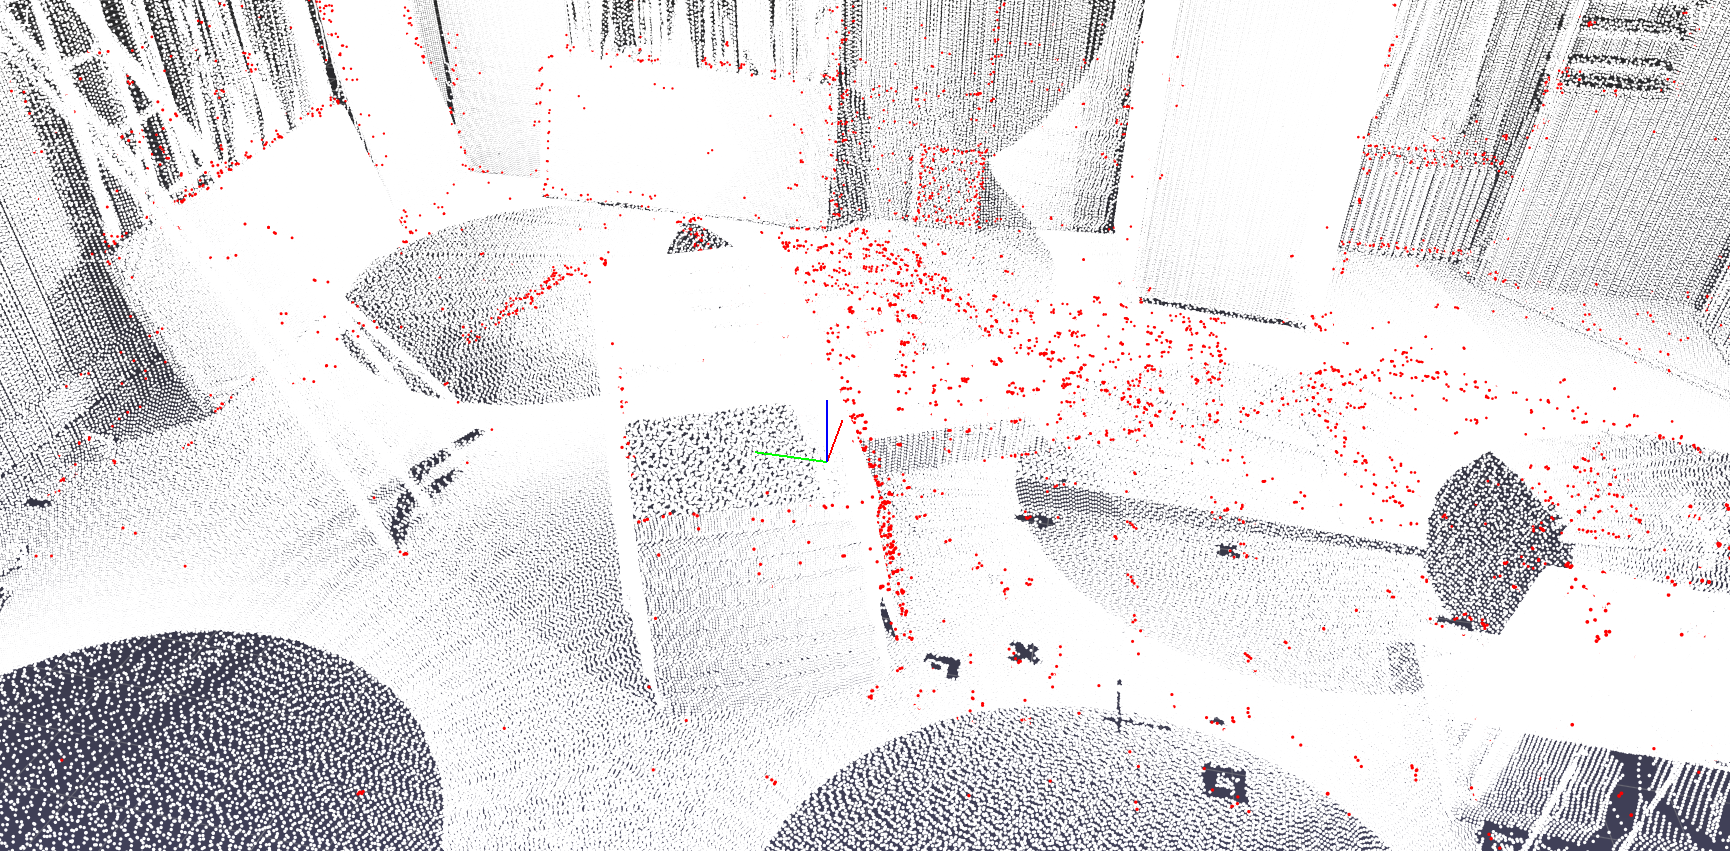
\includegraphics[width=4cm]{img/pointcloud_orb} }}%
    \qquad
    \subfloat[\centering DSM]{{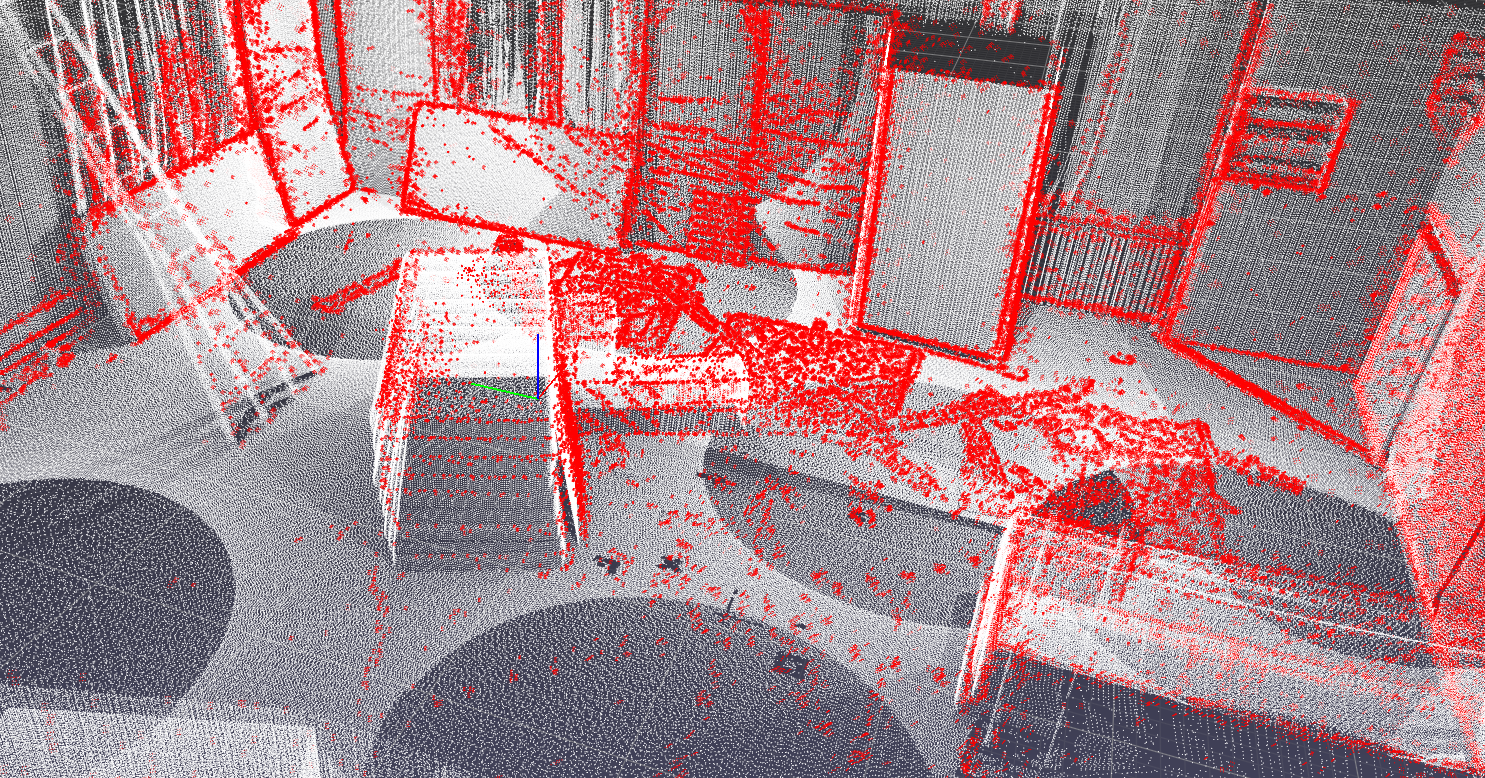
\includegraphics[width=4cm]{img/pointcloud_dsm} }}%
	\qquad
    \subfloat[\centering DSO]{{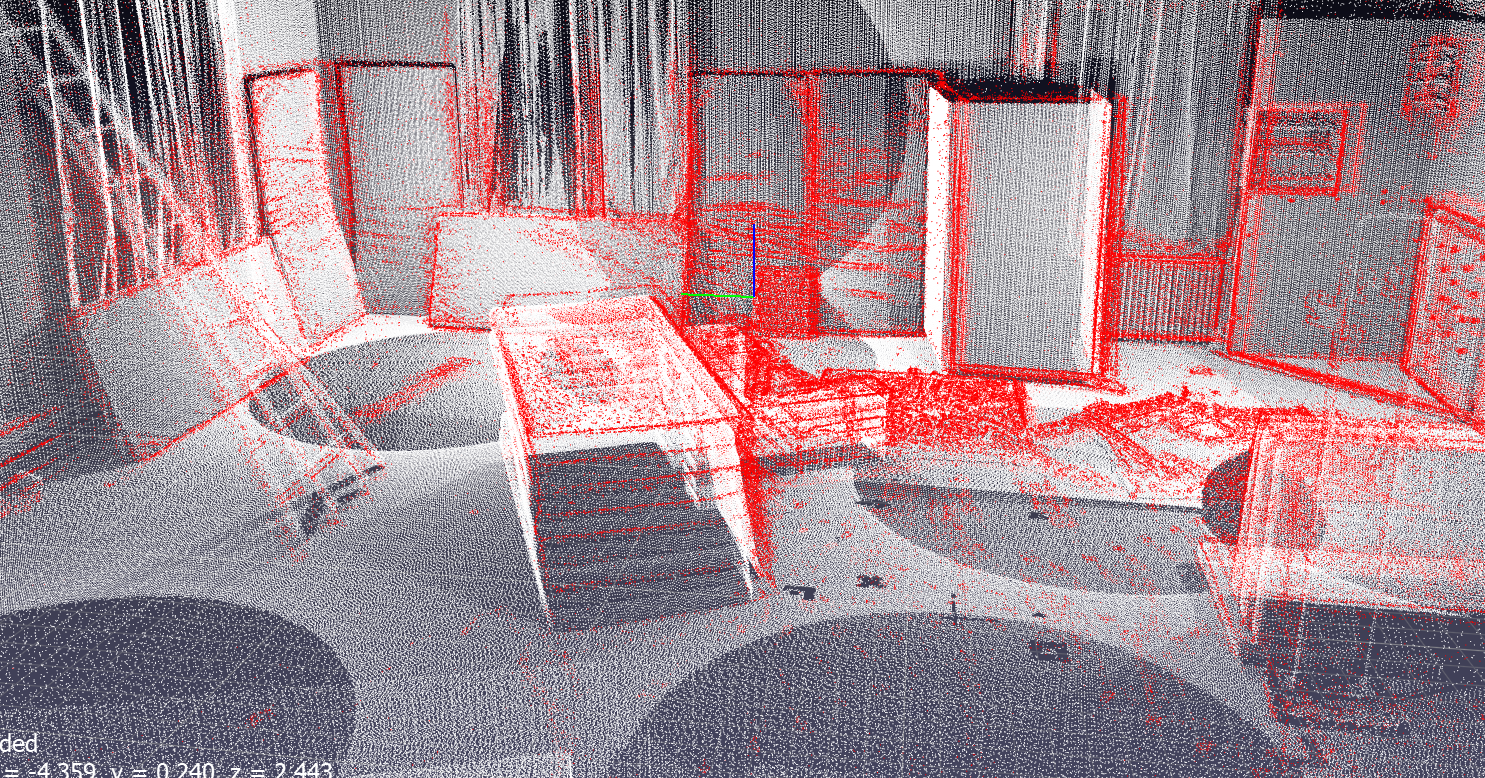
\includegraphics[width=4cm]{img/pointcloud_dso} }}%
    \caption{The groundtruth of the Pointcloud from Sequence V101 (white points) and the evaluated points by each algorithm (red points). 
	The points in Figure (a) are four times as large for better visability (ORB-SLAM generates only few points). 
	}%
    \label{fig:example}%
	\end{figure}

\section{Calculation Time}

